\documentclass{article}
\usepackage[utf8]{inputenc}
\usepackage{amsmath}
\usepackage{enumerate}
\usepackage{graphicx}
\usepackage{tikz}
\usetikzlibrary{bayesnet}
\usepackage{microtype}

\title{Topic Modeling Research}
\author{Melody Jiang}
\date{May 2019}

\begin{document}

\maketitle



\section{Possible Research Directions}


\subsection{Two main approaches to clustering}

\begin{enumerate}[(i)]
  \item \textbf{Distance-based} clustering. Using this approach, we analyze matrix of pairwise distances. Namely, suppose $y_i$ and $y_j$ are data points, then $D$ is a distance matrix whose $d_{ij}$ entry represents distance between $y_i$ and $y_j$.
  \item \textbf{Model-based} clustering. For example, $y_i \sim \sum_{h = 1}^k \pi_h \mathcal{K}(\theta_h)$.
\end{enumerate}


\subsection{Two main problems in clustering}

\begin{enumerate}[(i)]
  \item sensitivity to kernel
  \item issues in high dimensions (large p)
\end{enumerate}


\subsection{Semi-solutions}

\begin{enumerate}
  \item \textbf{C-Bayes}. All derivations from assumed models (e.g. kernel misspecification). See \cite{miller2018robust}.
  \item \textbf{Model plus distance-based clustering}.
  See \cite{duan2018bayesian}.
  \item \textbf{Calculating better distances}. E.g., geodesic or intrinsic distace (Didong Li \& Dunson, in preparation).
  \item \textbf{To address issues in high dimensions}, cluster on the latent variable level or varational autoencoder (VAE). 
\end{enumerate}



\section{Literature Review}

Three main tasks in textmining are clustering, classification, and information extraction \cite{allahyari2017brief}. Topic modeling can be applied to all of these tasks \cite{lu2011investigating}. We would like to focus on the most commonly used topic model, Latent Dirichlet Allocation (LDA), and LDA's robustness in the documeng clustering task. Lu et al. investigated LDA's task performance in document clustering and found LDA's performance is quite sensitive to the setting of its hyper-parameter and parameter \cite{lu2011investigating}. In terms of robustness, Wang et al. proposed a model-based approach to make LDA more robust by using localization and empirical Bayes \cite{wang2018general}.


\subsection{Viewpoints of document clustering}

\begin{itemize}
  \item hard clustering, soft clustering
  \item model-based clustering, distance-based clustering
  \item flat clustering, hierarchical clustering
  \item single group, multi-label
  \item special qualities of textdata and how traditional clustering algorithms are modified to accomodate for such speciality
\end{itemize}



\subsection{Latent Dirichlet Allocation (LDA)}

In this section, we reproduce the LDA model described in \cite{wang2018general} and \cite{blei2009topic}.

Let:

\begin{itemize}
  \item $K$ be a specified number of topics,
  \item $D$ the number of documents,
  \item $N_d$ the number of words in a document,
  \item $V$  the size of the vocabulary,
  \item $\boldsymbol{\alpha}$ a positive K-vector,
  \item $\eta$ a scalar. 
  \item $Dir_K(\boldsymbol{\alpha})$ a K-dimensional Dirichlet distribution with vector parameter $\boldsymbol{\alpha}$,
  \item $Dir_V(\eta)$ a V-Dimensional symmetric Dirichlet distribution with scalar parameter $\eta$.
\end{itemize}

A \textit{symmetric Dirichlet} is a Dirichlet distribution where each component of the parameter is equal to the same value.

We define each topic $\boldsymbol{\beta}_k$ to be a distribution over a fixed vocabulary and we fix the number of topics $K$. LDA assumes that a collection of documents comes from the following process:

\begin{enumerate}
  \item Draw each topic $\boldsymbol{\beta}_k \sim Dir_V(\eta)$ for k = 1, 2, ..., K.
  \item For each document $d$ ($d = 1, ..., D$),
  \begin{enumerate}
    \item Draw a vector of topic proportions $\boldsymbol{\theta}_d \sim Dir_K(\boldsymbol{\alpha})$
    \item For each word $w_n$ ($n = 1, ..., N_d$) in document $d$,
    \begin{enumerate}
      \item Draw topic assignment $z_{dn} \sim Mult(\boldsymbol{\theta}_d)$, where $z_{dn} \in \{1, ..., K\}$.
      \item Draw word $w_{dn} \sim Mult(\boldsymbol{\beta}_{z_{dn}})$, where $w_{dn} \in \{1, ..., V\}$.
    \end{enumerate}
  \end{enumerate}
\end{enumerate}

See Figure \ref{fig:gaphical_model_lda} for a directed graphical model of LDA.

\begin{figure}
  \centering
  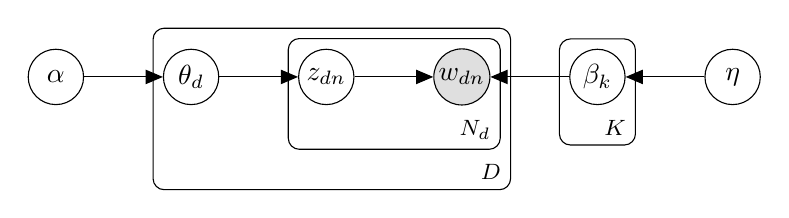
\begin{tikzpicture}

    % Nodes
    \node[obs] (w) {$w_{dn}$}; %word
    \node[latent, right=of w] (beta) {$\beta_k$}; %topic
    \node[latent, right=of beta] (eta) {$\eta$}; % eta
    \node[latent, left=of w] (z) {$z_{dn}$}; % topic assignment of word
    \node[latent, left=of z] (theta) {$\theta_d$}; % topic proportion of a document
    \node[latent, left=of theta] (alpha) {$\alpha$}; % hyperparameter alpha
  
    % Edge
    \edge {beta} {w}; % arrow pointing from topic to word
    \edge {eta} {beta}; % arrow pointing fromm eta to beta
    \edge {z} {w} % arrow pointing from topic assignment to word
    \edge {theta} {z} % arrow pointing from topic porportion of a document to topic assignment of a word
    \edge {alpha} {theta} % arrow pointing from hyperparameter alpha to topic proportion of a document
  
    % Plates
    \plate {wordPlate} {(w)(z)} {$N_d$};
    \plate {documentPlate} {(wordPlate)(theta)} {$D$};
    \plate {} {(beta)} {$K$};
  
  \end{tikzpicture}
  \caption{The directed graphical model of LDA. Adapted from \cite{blei2012probablistic} and \cite{blei2009topic}. Nodes denote random variables; edges denote dependence between random variables. Shaded nodes denote observed random variables; unshaded nodes denote hidden random variables. The rectangular boxes are ``plate notation", which denote replication.}
  \label{fig:gaphical_model_lda}
\end{figure}


\subsubsection{Likelihood functions of LDA}

\begin{align}
  p_d(w | \{\boldsymbol{\beta}_k\}_{1:K}, \boldsymbol{\theta}_d) = \sum_{k = 1}^K \theta_{dk} p(w | \boldsymbol{\beta}_k)
\end{align}

\begin{align}
  & p(d | \boldsymbol{\alpha}, \{\boldsymbol{\beta}_k\}_{1:K}) \\
  & = \int \left\{ \prod_{w \in V} \left[ \sum_{k = 1}^K \theta_{dk} p(w | \boldsymbol{\beta}_k) \right]^{c(w,d)} \right\} p(\boldsymbol{\theta}_d | \boldsymbol{\alpha}) d\boldsymbol{\theta}_d
\end{align}

Derivations are in appendix.



\subsection{Robust LDA}

In this section, we elaborate \cite{wang2018general}.


\subsubsection{Likelihood functions of Robust LDA}

\begin{align}
  & p(d | \boldsymbol{\alpha}, \{\boldsymbol{\beta}_k\}_{1:K}) \\
  & = \int \left\{ \prod_{w \in V} \left[ \sum_{k = 1}^K \theta_{dk} p(w | \boldsymbol{\beta}_{dk}) \right]^{c(w,d)} \right\} p(\boldsymbol{\theta}_d | \boldsymbol{\alpha}) d\boldsymbol{\theta}_d
\end{align}


\subsection{Evaluation}


\subsubsection{Evaluation of Clustering}

\begin{itemize}
  \item Internal criterion
  \item External criterion
  \begin{itemize}
    \item Purity
    \item Normalized mutual information (NMI)
    \item Rand index
    \item F measure
  \end{itemize}
\end{itemize}
\cite{manning2008iir}


\subsubsection{Evaluation of Topic Models}

Perplexity.


\section{Pilot Experiment}

In this section, we perform experiments similar to those in \cite{lu2011investigating}. We investigate how the hyperparameter $\alpha$ and the total number of topics $K$ affect LDA's performance in document clustering.

We use the Reuters-21578 R8 \footnote{https://www.cs.umb.edu/~smimarog/textmining/datasets/} dataset. Reuters-21578 R8 is a pre-processed subset of Reuters-21578, \footnote{http://www.daviddlewis.com/resources/testcollections/reuters21578/} a very widely used dataset in textmining research. Training data and testing data are provided in two separate files.

All analyses are done in R.

\subsection{Preprocessing}

First, we subset training data to 3 document classes (topics) for computational expense. We do the same for testing data.

Similar to what was done in \cite{lu2011investigating}, we study LDA in the standard clustering setting, where each document belongs to exactly one cluster. Hence, we remove documents appearing in two or more categories. Now we end up with 679 documents for training data and 279 documents for testing data.

As we have mentioned, Reuters-21578 R8 is a pre-processed subset of Reuters-21578. Preprocessing that has already been done for us are:

\begin{enumerate}
  \item Substituteing TAB, NEWLINE and RETURN characters by SPACE;
  \item Keeping only letters (i.e., turn punctuation, numbers, etc. into SPACES);
  \item Turning all letters to lowercase.
  \item Substituting multiple SPACES by a single SPACE.
  \item The title/subject of each document is simply added in the beginning of the document's text.
\end{enumerate}

Preprocessing steps performed by us are stopword removal and stemming. Tokenization is automatically performed when we create document-term matrices.


\subsection{Evaluation Metric}

We use perplexity of testing set as our evaluation metric, since the documents in the corpora are treated as if they were unlabeled. Perplexity is commonly used in topic modeling literature \cite{blei2003latent,blei2007correlated}. Other different evaluation metrics worth considering for future experiments include per-word predictive log likelihood used in \cite{wang2018general} and normalized mutual information used in \cite{lu2011investigating}.

As described in \cite{blei2003latent}, the perplexity is monotonically decrasing in the likelihood of the testing data, and perplexity is algebratically equivalent to the inverse of the geometric mean per-word likelihood. A lower perplexity score indicates better generalization performance of the model. For a testing dataset that consists of $M$ documents, the perplexity is:

$$
\text { perplexity }\left(D_{\text { test }}\right)=\exp \left\{-\frac{\sum_{d=1}^{M} \log p\left(\mathbf{w}_{d}\right)}{\sum_{d=1}^{M} N_{d}}\right\}
$$.


\subsection{Results}

First, using Gibbs sampling as estimation method, we calculate perplexity for $K = 2, 3, ..., 10$. $\alpha$ is estimated by the algorithm. See Figure \ref{fig:gibbs_diff_k_10} for result.

\begin{figure}[h]
  \centering
  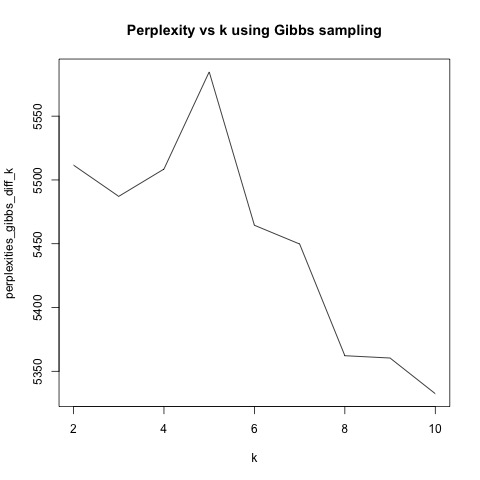
\includegraphics[width=0.5\linewidth]{images/gibbs_diff_k.jpg}
  \caption{Perplexity versus number of topics, Gibbs sampling}
  \label{fig:gibbs_diff_k_10}
\end{figure}

Then, using variational expectation-maximization (VEM) instead of Gibbs sampling as estimation method, we again calculate perplexity for $K = 2, 3, ..., 10$. $\alpha$ is still estimated by the algorithm. See Figure \ref{fig:vem_diff_k_10} for result.

\begin{figure}[h]
  \centering
  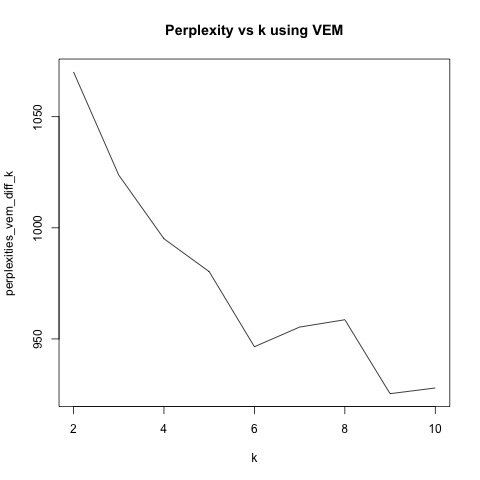
\includegraphics[width=0.5\linewidth]{images/vem_diff_k.jpg}
  \caption{Perplexity versus number of topics, VEM}
  \label{fig:vem_diff_k_10}
\end{figure}

At last, we use VEM as estimation method, fix the number of topics $K$ to be 3, and calculate perplexity for $\alpha = 0.01, 0.1, 1, 5, 10, 25$. Recall that we subsetted both training and testing data to be having 3 topics during preprocessing, so 3 is the actual number of topics for both training and testing data. See Figure \ref{fig:vem_diff_alpha} for results.

\begin{figure}[h]
  \centering
  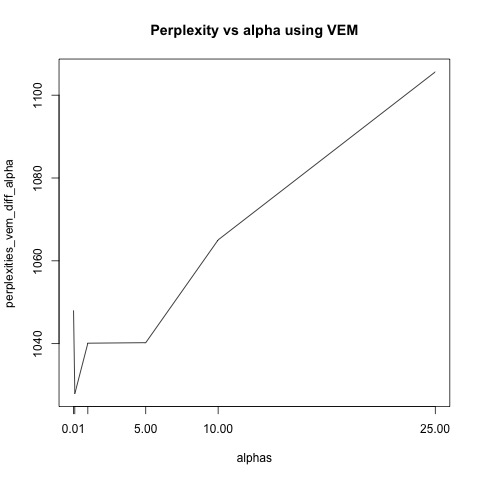
\includegraphics[width=0.5\linewidth]{images/vem_diff_alpha.jpg}
  \caption{Perplexity versus $\alpha$, VEM}
  \label{fig:vem_diff_alpha}
\end{figure}


\subsection{Discussion}

LDA is sensitive to the number of topics $K$ and the hyperparameter $\alpha$.

From Figure \ref{fig:gibbs_diff_k_10} and Figure \ref{fig:vem_diff_k_10}, we observe that the model tends to perform better with a larger number of topics, despite that the actual number of topics is 3. It may be worth investigating what causes this result - whether it is the nature of LDA, the evaluation method, or something else.

Figure \ref{fig:vem_diff_alpha} shows that LDA performs best when $\alpha$ is 0.1, and the performance worsen as $\alpha$ increases. This results agrees with the result in \cite{lu2011investigating}. The reason we obtain such result might be, as \cite{lu2011investigating} explained, while a larger value of $\alpha$ leads to more smoothed topics, $\alpha$ smaller than $1$ would cause the modes of the Dirichlet distribution to concentrate at corners of the simplex, thus favoring more sparse topics. Since we limited each document in our data to be in only one cluster, we would expect LDA to assgin a skewed topic distribution to a document. Therefore, a smaller $\alpha$ should result in better performance.







\section{Annotated Bibliography}
\cite{wang2018general}
Title: A general method for robust Bayesian Modeling.
This apaper proposes a general model-based approach to robustify Bayesian models.

\cite{doyle2009accounting}
Bursty Bayesian models.

\cite{blei2003latent}
Title: Latent dirichlet allocation.
An introduction to latent dirichlet allocation.

\cite{lu2011investigating}
Title: Investigating task performance of probabilistic topic models: an empirical study of PLSA and LDA. Investigates how alpha and k affect LDA's and PLSA's performance.

\cite{allahyari2017brief}
Title: A brief survey of text mining: Classification, clustering and extraction techniques

\cite{blei2007correlated}
Title: A correlated topic model of science. Used for justifying using perplexity as evalutation metric.


\section{Thoughts (for my own record)}

\begin{enumerate}
  \item document belonging to more than one category possible? Definitely - LDA is a mixture model. Other uses of topic model in text clustering? How are things often done in clustering research? 
  \item Outlier categories?
  \item To be investigated: More specific goal of analysis - what does document clustering really looklike?
\end{enumerate}



\section{Appendix}


\subsection{Derivations of Likelihood functions of LDA}


\bibliography{tm-bib}
\bibliographystyle{apalike}

\end{document}
